\documentclass[]{article}

\usepackage{graphicx}
\usepackage{placeins}
\usepackage{amsmath,amssymb}
\usepackage[colorlinks=true,citecolor=red]{hyperref}

\usepackage{geometry}
\geometry{a4paper,margin=1in,portrait}

\usepackage{tikz}
\usetikzlibrary{arrows,decorations.pathmorphing,backgrounds,positioning,fit}
\tikzset{module/.style={minimum size = 15mm,rectangle,draw=black,thick,fill=blue!20},
		pre/.style={<-,shorten <=1pt,>=stealth',semithick},
		post/.style={->,shorten <=1pt,>=stealth',semithick}}


\begin{document}
\title{Documentation for digital pattern generator-based imaging controller}
\author{Ryan Thomas}
\date{\today}
\maketitle

\section{Introduction}
\label{sec:introduction}
This document describes the design and operation of the digital pattern generator (DPG)-based imaging controller used in the Kj{\ae}rgaard lab.  While both this controller and its predecessor are implemented using a field-programmable gate array (FPGA), namely the Xlinx Spartan 3AN development board, the DPG imaging controller has a much simpler FPGA architecture and is more easily customizable than the previous, bespoke version.

Whereas the previous imaging controller had many different modules, each of which controlled a different aspect of the timing sequence, the DPG solution has only two modules: the DPG itself and a module to generate triggers for the FlexDDS.  The reason that these are separate is that we need millions of triggers for the FlexDDS at a fixed rate and duty cycle, and using a DPG to generate these would require an enormous amount of memory.  It is easier to use a dedicated module for this purpose.
\begin{figure}[htbp]
	\centering
	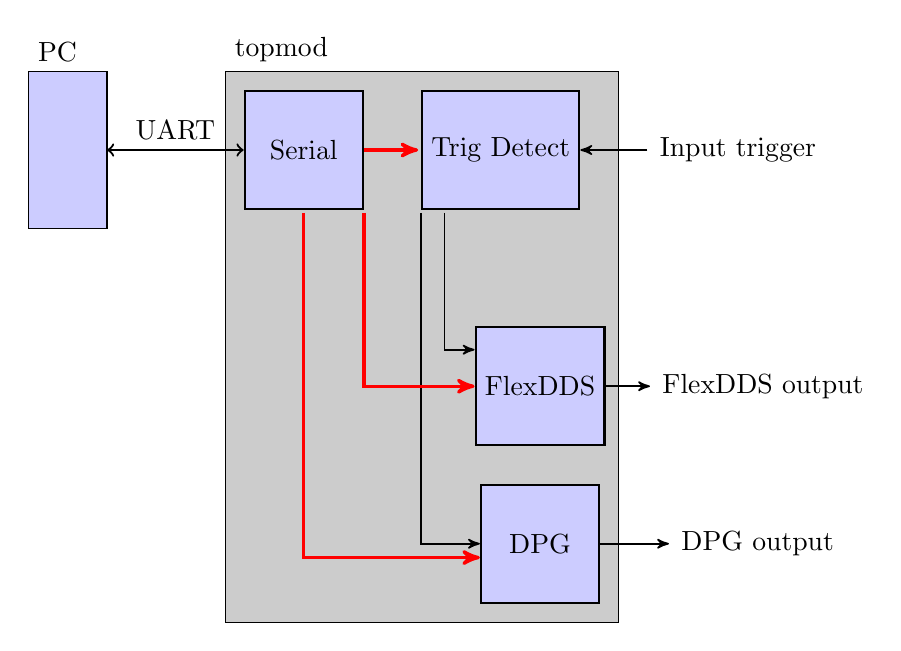
\begin{tikzpicture}
		\draw[fill=black!20] (0,0) rectangle (5,7);
		\node[anchor=south west] (topmod) at (0,7) {topmod};
		\draw[fill=blue!20] (-2.5,5) rectangle (-1.5,7);
		\node[anchor=south west] (pc) at (-2.5,7) {PC};
		\node[module] (serial) at (1,6) {Serial};
		\draw[<->,thick] (-1.5,6) -- node[above] {UART} (serial.west);
%		node[module] (serial) at ++(1,0) {Serial};
%		\node[module] (serial) at (1,6) {Serial} edge[pre] node[anchor=south] {UART} (pc);
		\node[module] (trig-detect) at (3.5,6) {Trig Detect} edge[pre,red,very thick] (serial);
		\node[module] (flexdds) at (4,3) {FlexDDS};
		\node[module] (dpg) at (4,1) {DPG};
		\draw[post] ([xshift=3mm]trig-detect.south west) |- ([yshift=-3mm]flexdds.north west);
		\draw[post] (trig-detect.south west) |- (dpg.west);
		\draw[post,red,very thick] (serial.south east) |- (flexdds.west);
		\draw[post,red,very thick] (serial.south) |- ([yshift=-5]dpg.west);
		
		\node[] (trigin) at ([xshift=2cm]trig-detect.east) {Input trigger} edge[post] (trig-detect.east);
		\node[] (flexdds-out) at ([xshift=2cm]flexdds.east) {FlexDDS output} edge[pre] (flexdds.east);
		\node[] (dpg-out) at ([xshift=2cm]dpg.east) {DPG output} edge[pre] (dpg.east);

	\end{tikzpicture}
	\caption{Diagram of the DPG-based imaging controller. A PC transmits parameters to the FlexDDS trigger generator and a digital pattern to the DPG.  The sequence starts either when an input trigger is received or when a software trigger is issued by the host PC over serial.  Thick red lines indicate the transmission of information to and from the serial controller.}
	\label{fg:diagram}
\end{figure}

\section{Digital Pattern Generator (DPG)}
\label{sec:dpg}
A DPG is simple to understand -- it is a device that stores a list of digital output patterns and the times at which they should be enacted.  In the case of the current DPG, these are stored as a series of 40-bit (5 byte) instructions, where the most-significant byte (MSB) is the type of instruction and bytes 0 to 3 (for a total of 32 bits) are the \emph{data}.  There are currently three types of instructions:
\begin{enumerate}
	\item $\mathrm{MSB} = 0\mathrm{x}00$ This instruction tells the DPG to wait for a time equal to \emph{data} sample clock cycles.
	\item $\mathrm{MSB} = 0\mathrm{x}01$ This instruction tells the DPG to output the pattern equal to \emph{data}.
	\item $\mathrm{MSB} = 0\mathrm{x}02$ This instruction tells the DPG to wait for a digital input event before continuing to the next instruction.  Bits 0 to 3 of \emph{data}, interpreted as an unsigned integer, indicate the digital input channel to look at, and bits 8 to 9 indicate the type of edge to look for.
\end{enumerate}

\begin{figure}
	\centering
	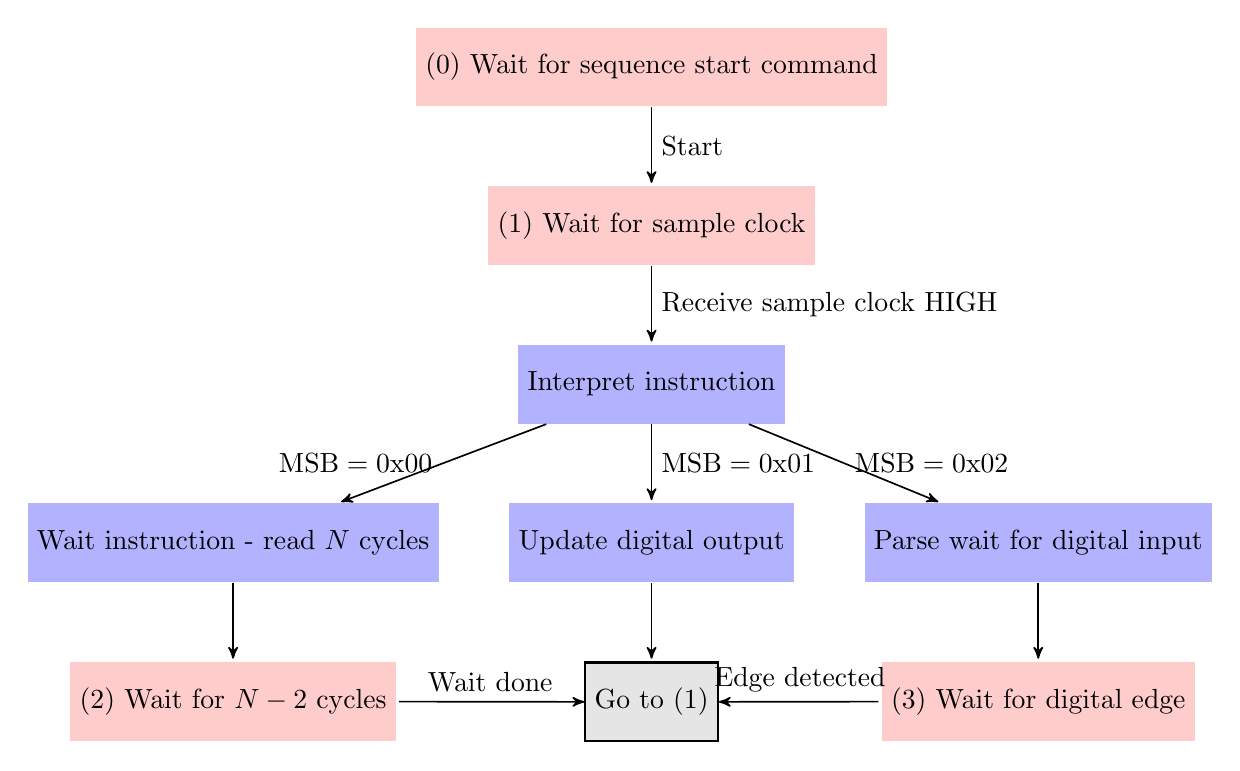
\begin{tikzpicture}[node distance=10mm and 10mm,
		state/.style={rectangle,fill=red!20,minimum size=10mm},
		cond/.style={rectangle,fill=blue!30,minimum size=10mm},
		goto/.style={rectangle,fill=black!10,draw=black,thick,minimum size=10mm}]
		\node[state] (wait-for-start) at (0,0) {(0) Wait for sequence start command};
		\node[state] (wait-for-sample-clock) [below=of wait-for-start] {(1) Wait for sample clock} edge[pre] node[anchor=west] {Start} (wait-for-start);
		\node[cond] (interpret-instruction) [below=of wait-for-sample-clock] {Interpret instruction} edge[pre] node[anchor=west] {Receive sample clock HIGH} (wait-for-sample-clock);
		
		\node[cond] (wait) [below left=of interpret-instruction] {Wait instruction - read $N$ cycles} edge[pre] node[anchor=east] {$\mathrm{MSB}=0\mathrm{x}00$} (interpret-instruction);
		\node[state] (wait-for) [below=of wait] {(2) Wait for $N-2$ cycles} edge[pre] node[anchor=east] {} (wait);
		
		\node[cond] (digital-out) [below=of interpret-instruction] {Update digital output}
		edge[pre] node[anchor=west] {$\mathrm{MSB}=0\mathrm{x}01$} (interpret-instruction);
		\node[goto] (goto-1) [below=of digital-out] {Go to (1)} edge[pre] (digital-out);
		\draw[post] (wait-for) -- node[above] {Wait done} (goto-1);
		
		\node[cond,node distance=10mm and 10mm] (wait-input) [below right=of interpret-instruction] {Parse wait for digital input} edge[pre] node[anchor=west] {$\mathrm{MSB}=0\mathrm{x}02$} (interpret-instruction);
		\node[state] (wait-edge) [below=of wait-input] {(3) Wait for digital edge} edge[pre] (wait-input);
		\draw[post] (wait-edge) -- node[above] {Edge detected} (goto-1);
		
%		\node[cond,node distance=10mm and 20mm] (seq-stop) [right=of wait-for-sample-clock] {Sequence stopped} edge[pre] node[anchor=south] {Empty instructions} (wait-for-sample-clock);
%		\draw[post] (seq-stop.north) |- (wait-for-start.east);
	\end{tikzpicture}
	\caption{Diagram of the finite-state machine (FSM) at the heart of the DPG.  Red boxes indicate states of the state machine; blue boxes indicate conditional statements.  New instructions are requested when a ``start'' command is received and also whenever a sample clock HIGH is detected.  When all instructions are read, the FSM returns to state 0, as well as when a sequence ``stop'' command is received.}
	\label{fg:dpg}
\end{figure}






\end{document}

